% Options for packages loaded elsewhere
\PassOptionsToPackage{unicode}{hyperref}
\PassOptionsToPackage{hyphens}{url}
%
\documentclass[
]{article}
\usepackage{amsmath,amssymb}
\usepackage{iftex}
\ifPDFTeX
  \usepackage[T1]{fontenc}
  \usepackage[utf8]{inputenc}
  \usepackage{textcomp} % provide euro and other symbols
\else % if luatex or xetex
  \usepackage{unicode-math} % this also loads fontspec
  \defaultfontfeatures{Scale=MatchLowercase}
  \defaultfontfeatures[\rmfamily]{Ligatures=TeX,Scale=1}
\fi
\usepackage{lmodern}
\ifPDFTeX\else
  % xetex/luatex font selection
\fi
% Use upquote if available, for straight quotes in verbatim environments
\IfFileExists{upquote.sty}{\usepackage{upquote}}{}
\IfFileExists{microtype.sty}{% use microtype if available
  \usepackage[]{microtype}
  \UseMicrotypeSet[protrusion]{basicmath} % disable protrusion for tt fonts
}{}
\makeatletter
\@ifundefined{KOMAClassName}{% if non-KOMA class
  \IfFileExists{parskip.sty}{%
    \usepackage{parskip}
  }{% else
    \setlength{\parindent}{0pt}
    \setlength{\parskip}{6pt plus 2pt minus 1pt}}
}{% if KOMA class
  \KOMAoptions{parskip=half}}
\makeatother
\usepackage{xcolor}
\usepackage[margin=1in]{geometry}
\usepackage{color}
\usepackage{fancyvrb}
\newcommand{\VerbBar}{|}
\newcommand{\VERB}{\Verb[commandchars=\\\{\}]}
\DefineVerbatimEnvironment{Highlighting}{Verbatim}{commandchars=\\\{\}}
% Add ',fontsize=\small' for more characters per line
\usepackage{framed}
\definecolor{shadecolor}{RGB}{248,248,248}
\newenvironment{Shaded}{\begin{snugshade}}{\end{snugshade}}
\newcommand{\AlertTok}[1]{\textcolor[rgb]{0.94,0.16,0.16}{#1}}
\newcommand{\AnnotationTok}[1]{\textcolor[rgb]{0.56,0.35,0.01}{\textbf{\textit{#1}}}}
\newcommand{\AttributeTok}[1]{\textcolor[rgb]{0.13,0.29,0.53}{#1}}
\newcommand{\BaseNTok}[1]{\textcolor[rgb]{0.00,0.00,0.81}{#1}}
\newcommand{\BuiltInTok}[1]{#1}
\newcommand{\CharTok}[1]{\textcolor[rgb]{0.31,0.60,0.02}{#1}}
\newcommand{\CommentTok}[1]{\textcolor[rgb]{0.56,0.35,0.01}{\textit{#1}}}
\newcommand{\CommentVarTok}[1]{\textcolor[rgb]{0.56,0.35,0.01}{\textbf{\textit{#1}}}}
\newcommand{\ConstantTok}[1]{\textcolor[rgb]{0.56,0.35,0.01}{#1}}
\newcommand{\ControlFlowTok}[1]{\textcolor[rgb]{0.13,0.29,0.53}{\textbf{#1}}}
\newcommand{\DataTypeTok}[1]{\textcolor[rgb]{0.13,0.29,0.53}{#1}}
\newcommand{\DecValTok}[1]{\textcolor[rgb]{0.00,0.00,0.81}{#1}}
\newcommand{\DocumentationTok}[1]{\textcolor[rgb]{0.56,0.35,0.01}{\textbf{\textit{#1}}}}
\newcommand{\ErrorTok}[1]{\textcolor[rgb]{0.64,0.00,0.00}{\textbf{#1}}}
\newcommand{\ExtensionTok}[1]{#1}
\newcommand{\FloatTok}[1]{\textcolor[rgb]{0.00,0.00,0.81}{#1}}
\newcommand{\FunctionTok}[1]{\textcolor[rgb]{0.13,0.29,0.53}{\textbf{#1}}}
\newcommand{\ImportTok}[1]{#1}
\newcommand{\InformationTok}[1]{\textcolor[rgb]{0.56,0.35,0.01}{\textbf{\textit{#1}}}}
\newcommand{\KeywordTok}[1]{\textcolor[rgb]{0.13,0.29,0.53}{\textbf{#1}}}
\newcommand{\NormalTok}[1]{#1}
\newcommand{\OperatorTok}[1]{\textcolor[rgb]{0.81,0.36,0.00}{\textbf{#1}}}
\newcommand{\OtherTok}[1]{\textcolor[rgb]{0.56,0.35,0.01}{#1}}
\newcommand{\PreprocessorTok}[1]{\textcolor[rgb]{0.56,0.35,0.01}{\textit{#1}}}
\newcommand{\RegionMarkerTok}[1]{#1}
\newcommand{\SpecialCharTok}[1]{\textcolor[rgb]{0.81,0.36,0.00}{\textbf{#1}}}
\newcommand{\SpecialStringTok}[1]{\textcolor[rgb]{0.31,0.60,0.02}{#1}}
\newcommand{\StringTok}[1]{\textcolor[rgb]{0.31,0.60,0.02}{#1}}
\newcommand{\VariableTok}[1]{\textcolor[rgb]{0.00,0.00,0.00}{#1}}
\newcommand{\VerbatimStringTok}[1]{\textcolor[rgb]{0.31,0.60,0.02}{#1}}
\newcommand{\WarningTok}[1]{\textcolor[rgb]{0.56,0.35,0.01}{\textbf{\textit{#1}}}}
\usepackage{graphicx}
\makeatletter
\def\maxwidth{\ifdim\Gin@nat@width>\linewidth\linewidth\else\Gin@nat@width\fi}
\def\maxheight{\ifdim\Gin@nat@height>\textheight\textheight\else\Gin@nat@height\fi}
\makeatother
% Scale images if necessary, so that they will not overflow the page
% margins by default, and it is still possible to overwrite the defaults
% using explicit options in \includegraphics[width, height, ...]{}
\setkeys{Gin}{width=\maxwidth,height=\maxheight,keepaspectratio}
% Set default figure placement to htbp
\makeatletter
\def\fps@figure{htbp}
\makeatother
\setlength{\emergencystretch}{3em} % prevent overfull lines
\providecommand{\tightlist}{%
  \setlength{\itemsep}{0pt}\setlength{\parskip}{0pt}}
\setcounter{secnumdepth}{-\maxdimen} % remove section numbering
\ifLuaTeX
  \usepackage{selnolig}  % disable illegal ligatures
\fi
\IfFileExists{bookmark.sty}{\usepackage{bookmark}}{\usepackage{hyperref}}
\IfFileExists{xurl.sty}{\usepackage{xurl}}{} % add URL line breaks if available
\urlstyle{same}
\hypersetup{
  pdftitle={Lab 2 Assignment},
  pdfauthor={Evan O'Toole},
  hidelinks,
  pdfcreator={LaTeX via pandoc}}

\title{Lab 2 Assignment}
\author{Evan O'Toole}
\date{Feb 14th, 2025}

\begin{document}
\maketitle

\hypertarget{general-instructions}{%
\section{General Instructions}\label{general-instructions}}

\begin{itemize}
\tightlist
\item
  Put your name in the author section and fill in the date section
  above.
\item
  Write R code in the R chunks provided to answer the questions
  posed.Always print your results to the question.
\item
  You may use any code/materials, including past lab materials, on
  Brightspace.
\item
  Execute each chunk of code to ensure that your code works properly.
\item
  If you cannot compile all of your code without errors before the end
  of the lab, comment out the chunks that are not working.
\item
  Save the Rmd file in your personal directory (refer to Lab 0
  instructions if needed).
\item
  Knit to PDF (or Word/HTML, but then print those to PDF).
\item
  Upload the PDF file to Brightspace.
\end{itemize}

\hypertarget{the-data}{%
\section{The Data}\label{the-data}}

Suppose a city council was interested in improving accessibility to
public amenities. They want to count the number of public restrooms
available in their downtown area per city block. They sample 12 blocks
and count the number of restrooms per city block. If the locations of
restrooms are random, then a Poisson(lambda) model should be appropriate
for the data.

\begin{Shaded}
\begin{Highlighting}[]
\NormalTok{pdat }\OtherTok{\textless{}{-}} \FunctionTok{c}\NormalTok{(}\DecValTok{1}\NormalTok{, }\DecValTok{6}\NormalTok{, }\DecValTok{1}\NormalTok{, }\DecValTok{2}\NormalTok{, }\DecValTok{0}\NormalTok{, }\DecValTok{1}\NormalTok{, }\DecValTok{5}\NormalTok{, }\DecValTok{1}\NormalTok{, }\DecValTok{4}\NormalTok{, }\DecValTok{3}\NormalTok{, }\DecValTok{3}\NormalTok{, }\DecValTok{0}\NormalTok{)}
\NormalTok{lambda\_mle }\OtherTok{\textless{}{-}} \FunctionTok{mean}\NormalTok{(pdat)}

\CommentTok{\# Create a sequence of lambda values from 1 to 6 in steps of 0.05}
\NormalTok{lambda\_seq }\OtherTok{\textless{}{-}} \FunctionTok{seq}\NormalTok{(}\DecValTok{1}\NormalTok{, }\DecValTok{6}\NormalTok{, }\FloatTok{0.05}\NormalTok{)}
\end{Highlighting}
\end{Shaded}

\hypertarget{compute-sample-mean-and-create-lambda-sequence}{%
\section{1. Compute Sample Mean and Create Lambda
Sequence}\label{compute-sample-mean-and-create-lambda-sequence}}

The sample mean of \texttt{pdat} is the MLE of lambda given this data.
Then create a sequence of lambda values from 1 to 6 in steps of 0.05.

\begin{Shaded}
\begin{Highlighting}[]
\CommentTok{\# Define the log{-}likelihood function for the Poisson distribution}
\NormalTok{log\_likelihood }\OtherTok{\textless{}{-}} \ControlFlowTok{function}\NormalTok{(lambda, x) \{}
\NormalTok{  loglike }\OtherTok{\textless{}{-}} \DecValTok{0}
  \ControlFlowTok{for}\NormalTok{ (i }\ControlFlowTok{in} \DecValTok{1}\SpecialCharTok{:}\FunctionTok{length}\NormalTok{(x)) \{}
\NormalTok{    loglike }\OtherTok{\textless{}{-}}\NormalTok{ loglike }\SpecialCharTok{+} \FunctionTok{dpois}\NormalTok{(x[i], lambda, }\AttributeTok{log =} \ConstantTok{TRUE}\NormalTok{)  }\CommentTok{\# Sum of log of Poisson PMF}
\NormalTok{  \}}
  \FunctionTok{return}\NormalTok{(loglike)}
\NormalTok{\}}

\CommentTok{\# Compute the log{-}likelihood for each value of lambda, given data \textasciigrave{}pdat\textasciigrave{}}
\NormalTok{loglike\_vals }\OtherTok{\textless{}{-}} \FunctionTok{sapply}\NormalTok{(lambda\_seq, }\ControlFlowTok{function}\NormalTok{(l) }\FunctionTok{log\_likelihood}\NormalTok{(l, pdat))}

\CommentTok{\# Show the first few values of lambda and corresponding log{-}likelihoods}
\FunctionTok{head}\NormalTok{(}\FunctionTok{cbind}\NormalTok{(lambda\_seq, loglike\_vals))}
\end{Highlighting}
\end{Shaded}

\begin{verbatim}
##      lambda_seq loglike_vals
## [1,]       1.00    -30.82146
## [2,]       1.05    -30.10413
## [3,]       1.10    -29.44809
## [4,]       1.15    -28.84789
## [5,]       1.20    -28.29878
## [6,]       1.25    -27.79659
\end{verbatim}

\begin{Shaded}
\begin{Highlighting}[]
\CommentTok{\# Plot the log{-}likelihood values against lambda}
\FunctionTok{plot}\NormalTok{(loglike\_vals }\SpecialCharTok{\textasciitilde{}}\NormalTok{ lambda\_seq, }\AttributeTok{ylab =} \StringTok{\textquotesingle{}Log{-}Likelihood\textquotesingle{}}\NormalTok{, }\AttributeTok{xlab =} \StringTok{\textquotesingle{}lambda (Rate)\textquotesingle{}}\NormalTok{, }\AttributeTok{type =} \StringTok{\textquotesingle{}l\textquotesingle{}}\NormalTok{)}

\CommentTok{\# Add a title with the correct value of n}
\NormalTok{n }\OtherTok{\textless{}{-}} \FunctionTok{length}\NormalTok{(pdat)  }\CommentTok{\# Number of observations}
\FunctionTok{title}\NormalTok{(}\FunctionTok{paste}\NormalTok{(}\StringTok{\textquotesingle{}Poisson Log{-}likelihood for n=\textquotesingle{}}\NormalTok{, n, }\AttributeTok{sep=}\StringTok{\textquotesingle{}\textquotesingle{}}\NormalTok{))}
\end{Highlighting}
\end{Shaded}

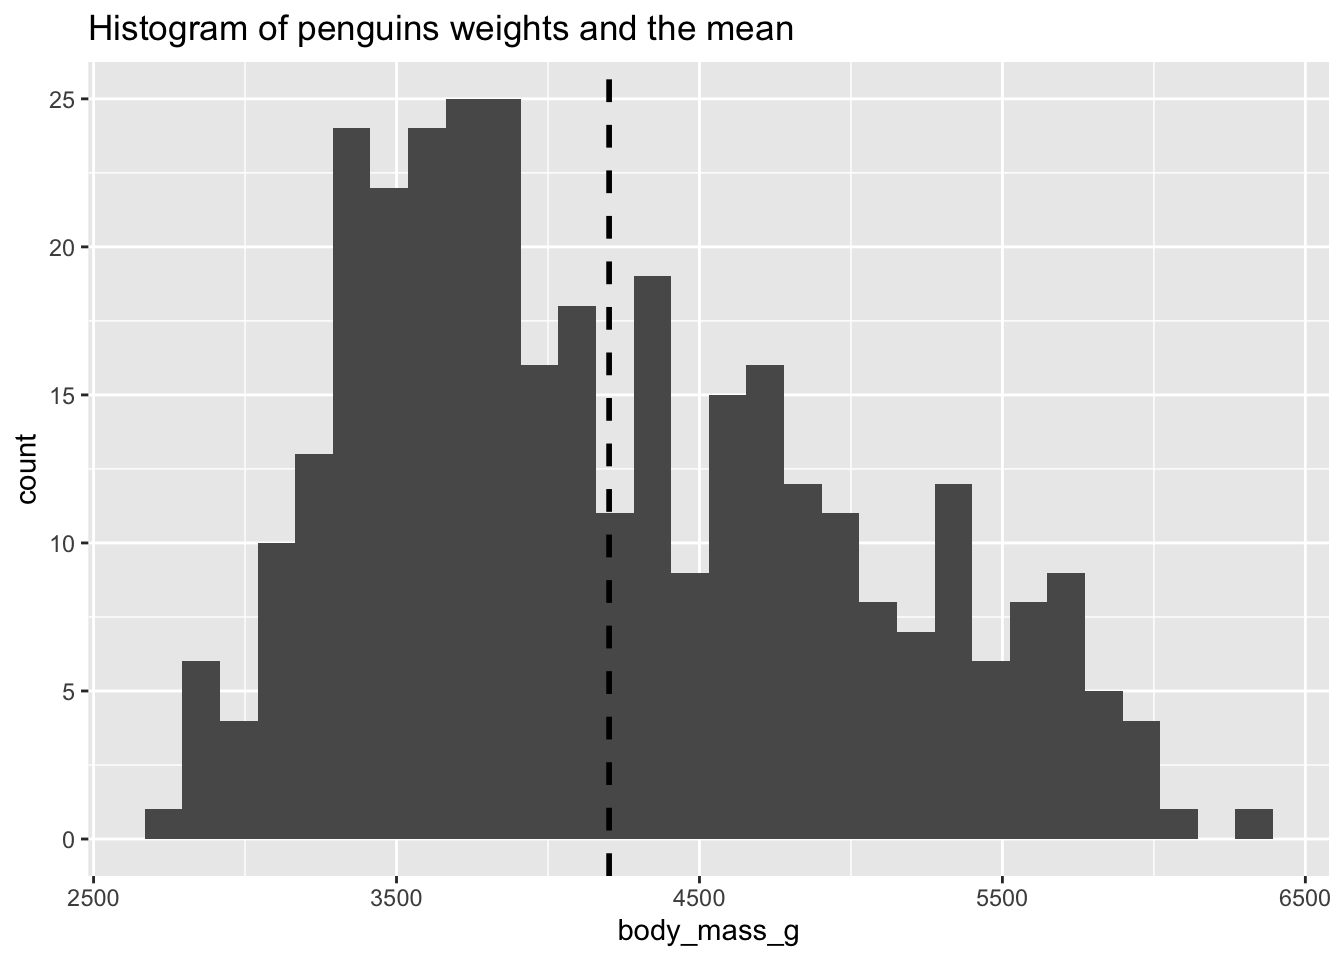
\includegraphics{Lab2-Assignment_files/figure-latex/unnamed-chunk-2-1.pdf}

\hypertarget{compute-mle-of-the-log-likelihood-function-using-optimize}{%
\section{3. Compute MLE of the Log-Likelihood Function using
optimize()}\label{compute-mle-of-the-log-likelihood-function-using-optimize}}

\begin{Shaded}
\begin{Highlighting}[]
\CommentTok{\# Find the MLE of lambda using optimize()}
\NormalTok{result }\OtherTok{\textless{}{-}} \FunctionTok{optimize}\NormalTok{(log\_likelihood, }\AttributeTok{interval =} \FunctionTok{c}\NormalTok{(}\FloatTok{0.0001}\NormalTok{, }\DecValTok{15}\NormalTok{), }\AttributeTok{maximum =} \ConstantTok{TRUE}\NormalTok{, }\AttributeTok{x =}\NormalTok{ pdat)}
\NormalTok{lambda\_hat }\OtherTok{\textless{}{-}}\NormalTok{ result}\SpecialCharTok{$}\NormalTok{maximum  }\CommentTok{\# MLE of lambda}
\NormalTok{lambda\_hat  }\CommentTok{\# Display the MLE of lambda}
\end{Highlighting}
\end{Shaded}

\begin{verbatim}
## [1] 2.249999
\end{verbatim}

\hypertarget{log-relative-likelihood-minus-lnp-function-and-plot}{%
\section{4. Log Relative Likelihood Minus ln(p) Function and
Plot}\label{log-relative-likelihood-minus-lnp-function-and-plot}}

Write a function to compute the log relative likelihood minus ln(p).
Plot the function against the lambda sequence you created in part 3,
using p=0.1. Your plot must have an appropriate title and labelled axes.
Include a horizontal line at y=0, set the color of the line to be red.

\begin{Shaded}
\begin{Highlighting}[]
\CommentTok{\# Log relative likelihood function}
\NormalTok{log\_relative\_likelihood }\OtherTok{\textless{}{-}} \ControlFlowTok{function}\NormalTok{(lambda, lambda\_hat, x) \{}
  \FunctionTok{log\_likelihood}\NormalTok{(lambda, x) }\SpecialCharTok{{-}} \FunctionTok{log\_likelihood}\NormalTok{(lambda\_hat, x)}
\NormalTok{\}}

\CommentTok{\# Log relative likelihood minus ln(p) function}
\NormalTok{log\_relative\_likelihood\_minus\_ln\_p }\OtherTok{\textless{}{-}} \ControlFlowTok{function}\NormalTok{(lambda, lambda\_hat, x, p) \{}
  \FunctionTok{log\_relative\_likelihood}\NormalTok{(lambda, lambda\_hat, x) }\SpecialCharTok{{-}} \FunctionTok{log}\NormalTok{(p)}
\NormalTok{\}}

\CommentTok{\# Set the threshold for 10\% likelihood (p = 0.1)}
\NormalTok{p }\OtherTok{\textless{}{-}} \FloatTok{0.1}

\CommentTok{\# Plot the log relative likelihood minus ln(p) function against lambda}
\FunctionTok{plot}\NormalTok{(}\FunctionTok{log\_relative\_likelihood\_minus\_ln\_p}\NormalTok{(lambda\_seq, lambda\_hat, pdat, p) }\SpecialCharTok{\textasciitilde{}}\NormalTok{ lambda\_seq, }
     \AttributeTok{ylab =} \StringTok{\textquotesingle{}r(lambda) {-} ln(p)\textquotesingle{}}\NormalTok{, }\AttributeTok{xlab =} \StringTok{\textquotesingle{}lambda\textquotesingle{}}\NormalTok{, }\AttributeTok{type =} \StringTok{\textquotesingle{}l\textquotesingle{}}\NormalTok{)}

\CommentTok{\# Add a horizontal line at y = 0 to indicate the likelihood threshold}
\FunctionTok{abline}\NormalTok{(}\AttributeTok{h =} \DecValTok{0}\NormalTok{, }\AttributeTok{col =} \StringTok{"red"}\NormalTok{, }\AttributeTok{lty =} \DecValTok{2}\NormalTok{)}

\CommentTok{\# Add a title}
\FunctionTok{title}\NormalTok{(}\StringTok{\textquotesingle{}Log Relative Likelihood for 10\% Likelihood Interval\textquotesingle{}}\NormalTok{)}
\end{Highlighting}
\end{Shaded}

\includegraphics{Lab2-Assignment_files/figure-latex/unnamed-chunk-4-1.pdf}

\hypertarget{compute-10-likelihood-interval-using-uniroot}{%
\section{5. Compute 10\% Likelihood Interval using
uniroot()}\label{compute-10-likelihood-interval-using-uniroot}}

\begin{Shaded}
\begin{Highlighting}[]
\NormalTok{p }\OtherTok{\textless{}{-}} \FloatTok{0.1}

\CommentTok{\# Use uniroot to find the lower bound of the 10\% likelihood interval}
\NormalTok{lower\_interval }\OtherTok{\textless{}{-}} \FunctionTok{uniroot}\NormalTok{(log\_relative\_likelihood\_minus\_ln\_p, }
                          \FunctionTok{c}\NormalTok{(}\DecValTok{1}\NormalTok{, }\DecValTok{2}\NormalTok{), }\AttributeTok{lambda\_hat =}\NormalTok{ lambda\_hat, }\AttributeTok{x =}\NormalTok{ pdat, }\AttributeTok{p =}\NormalTok{ p)}
\NormalTok{lower\_root }\OtherTok{\textless{}{-}}\NormalTok{ lower\_interval}\SpecialCharTok{$}\NormalTok{root  }\CommentTok{\# Lower bound of the 10\% likelihood interval}

\CommentTok{\# Use uniroot to find the upper bound of the 10\% likelihood interval}
\NormalTok{upper\_interval }\OtherTok{\textless{}{-}} \FunctionTok{uniroot}\NormalTok{(log\_relative\_likelihood\_minus\_ln\_p, }
                          \FunctionTok{c}\NormalTok{(}\DecValTok{3}\NormalTok{, }\DecValTok{15}\NormalTok{), }\AttributeTok{lambda\_hat =}\NormalTok{ lambda\_hat, }\AttributeTok{x =}\NormalTok{ pdat, }\AttributeTok{p =}\NormalTok{ p)}
\NormalTok{upper\_root }\OtherTok{\textless{}{-}}\NormalTok{ upper\_interval}\SpecialCharTok{$}\NormalTok{root  }\CommentTok{\# Upper bound of the 10\% likelihood interval}

\CommentTok{\# Display the roots}
\NormalTok{lower\_root}
\end{Highlighting}
\end{Shaded}

\begin{verbatim}
## [1] 1.444032
\end{verbatim}

\begin{Shaded}
\begin{Highlighting}[]
\NormalTok{upper\_root}
\end{Highlighting}
\end{Shaded}

\begin{verbatim}
## [1] 3.311317
\end{verbatim}

\end{document}
